%!TEX root = main.tex
\section{Towards Dataset Understanding\label{sec:understanding}}
One of the key goal of visual data exploration is to -----  understanding of the dataset. While the ---- discussed in the last few sections have assumed that the user has some knowleldge of what he is interested in. This section discusses the ------ providing recommendations and continual provenance without explicit signals from the user. This can happen in two scenarios: 1) user is at the beginning of their analysis  2) user doesn't know what to query for. The two scenarios are not mutually exclusive. The former is the well-known cold-start problem in recommender system. The latter is less well-known and derived from our finding in Section~\ref{sec:hypothesis}. 

In this section, we will first describe \sbd, a system that provides data summaries. Then we will discuss the challenges ahead and opportunities in this space.
\subsection{\sbd: Navigating Through Data Slices with Hierarchical Summary of Visualizations}
%understanding distributions (distribution awareness)
%introduce problem + challenge
\par Common analytics tasks, such as causal inference, feature selection, and outlier detection requires studying the distributions or patterns at different levels of data granularity~\cite{Anand2015,Wu2013,Heer2012}. However, without knowing \textit{what} subset of data contains an insightful distribution, manually exploring distributions from all possible data subsets can be tedious and inefficient. In order to explore different data subsets, a user would first have to construct a large number of visualizations corresponding to all possible data subsets, and then, navigating through this large space of visualizations to draw meaningful insights
%there is no systematic way to perform these exercises.
% explain what storyboard does
\par To this end, we present \sbd, an interactive visualization summarization system that automatically selects a small set of visualizations to summarize the distributions within a dataset in an informative manner. Figure~\ref{sbd} illustrates a example dashboard generated by \sbd from the Police Stop Dataset \cite{police}, which contains records of police stops that resulted in a warning, ticket, or an arrest. The attributes in the dataset include driver gender, age, race, and the stop time of day, whether a search was conducted, and whether contraband was found. We request \sbd to generate a dashboard of 9 visualizations with bar charts with x-axis as the stop outcome (whether the police stop resulted in a ticket, warning, or arrest/summons) and y-axis as the percentage of police stops that led to this outcome. First, at the top of our dashboard, \sbd highlights three key data subsets that results in a high arrest rate, which looks very different trend than the overall (where the majority of stops results in tickets). Following along the leftmost branch, we learn that even though in general when a search is conducted, the arrest rate is almost as high as ticketing rate, when we look at the asian population, whether a search is conducted had less influence on the arrest rate and the trend resembles more like the overall distribution.

\begin{figure}[h!]
\label{fig:sbd}
\centering
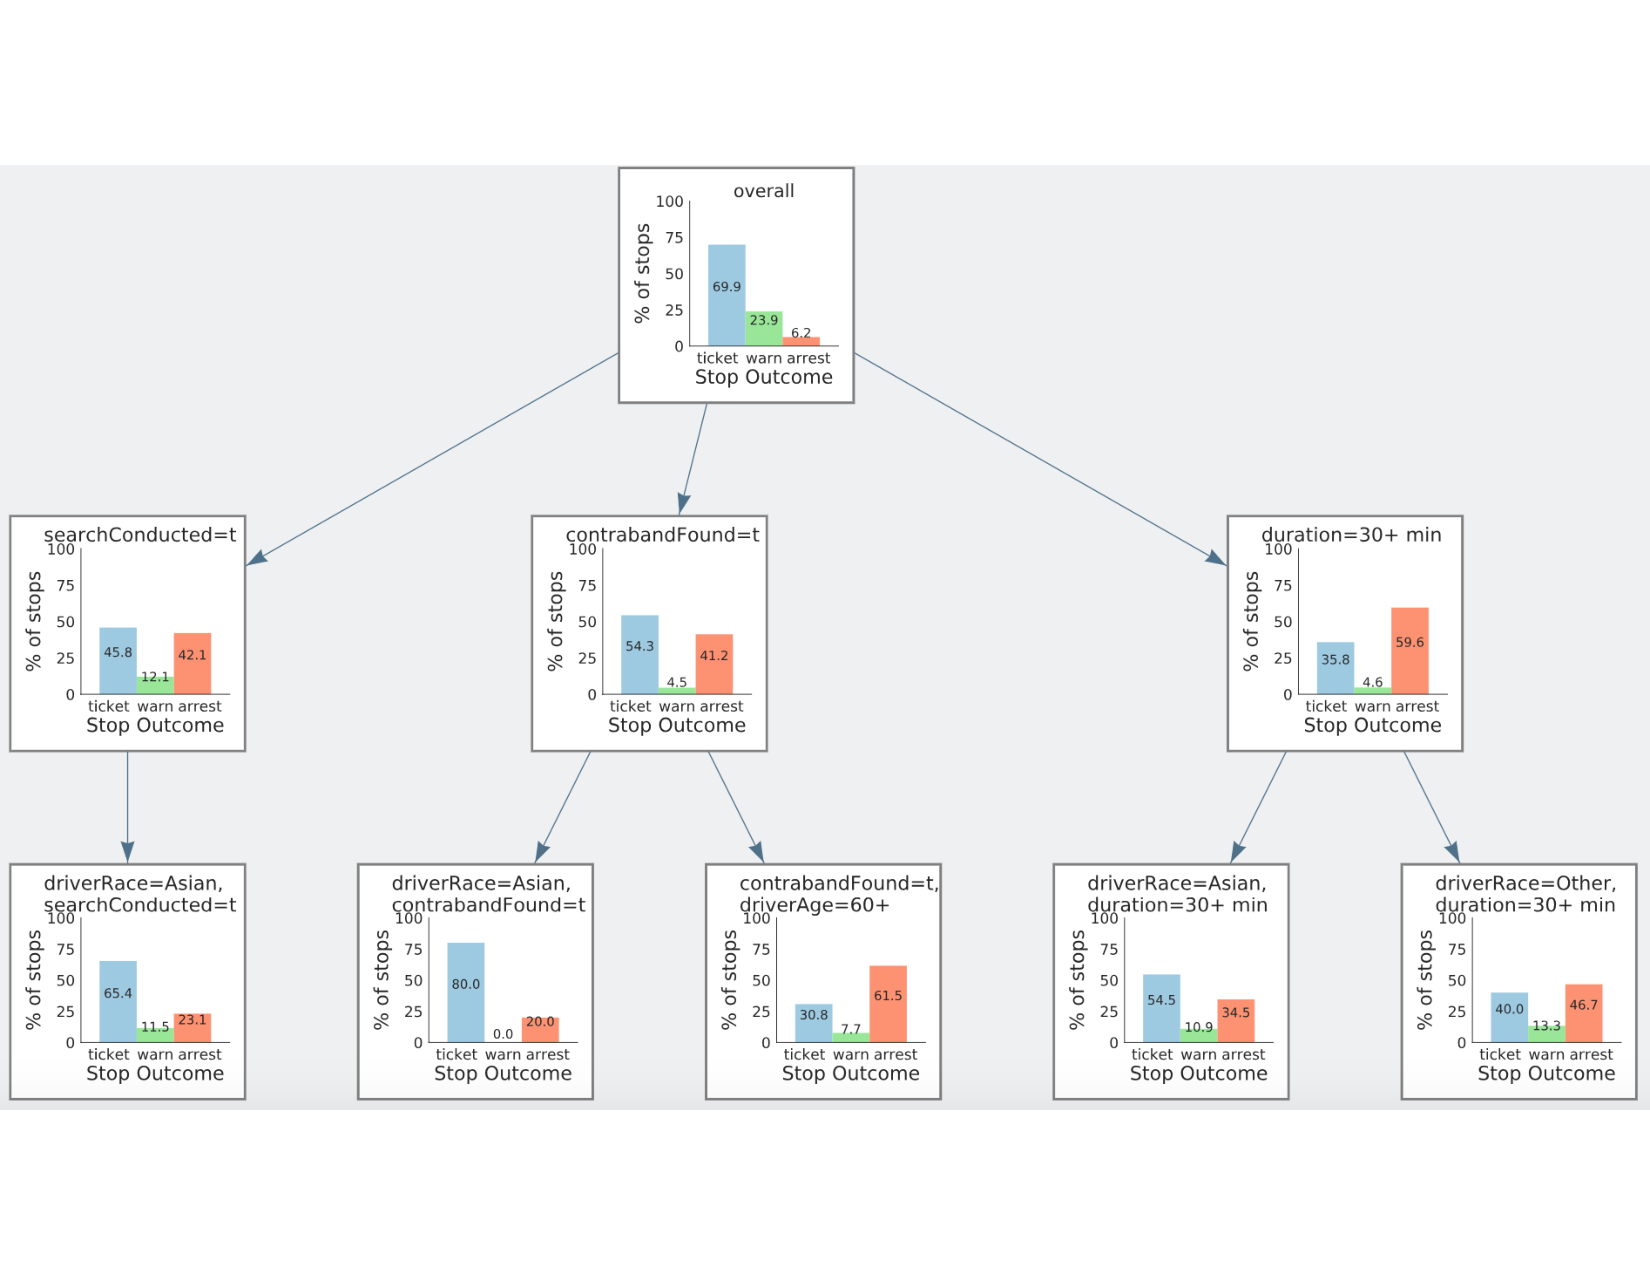
\includegraphics[width=0.7\linewidth]{figures/storyboard.pdf}
\caption{Example dashboard generated by \sbd summarizing the key insights in the Police dataset.}
\end{figure} 

Nevertheless, finding effective visualizations to summarize a dataset is not as trivial as picking individual visualizations that maximizes some statistical measure, such as deviation~\cite{Vartak2015}, coverage~\cite{Sarvghad2017}, or significance testing~\cite{Anand2015}, which can often result in misleading summarizations. The above example demonstrates a scenario where the selection of an improper reference (female) for comparing the visualization (black female) against results in misleading insights. In \sbd, we formulate an objective where a visualization is \emph{actually} interesting when it deviates from and can not be explained by \emph{even} its most informative reference.
% one paragraph on motivation on objectives and explain lattice + traversal 




%explain distribution awareness + its application, its relationship with dataset understnading + how it can be used in other contexts.
\par Our user study show that \sbd guides users to make better predictions regarding unseen visualizations, ranking attribute importance, and retreival of interesting visualizations compared to the baselines. The effectiveness of \sbd largely comes from how it helps analysts become more \emph{distributionally aware} of the dataset. We define \emph{distribution awareness} as the aspect of data understanding in which analysts make sense of the key distributions across different data subsets and their relationship in the context of the dataset. Even though it may be infeasible to examine all possible data subsets, with distribution awareness, the analyst will still be able to draw meaningful insights and establish correlations about related visualizations by generalizing their understanding to make predictions regarding the unseen visualizations. 

How ----- is underexplored 
future research 
building systems that ---
can effectively guide analysts towards more meaningful stories for further investigation.
discussed next.
\subsection{Challenges Ahead}
Recommendation providing better understanding for overall dataset and understanding. For example, \zv displays representative and outlier patterns to help provide
an overview of typical trends for the data to be queried. 

\begin{itemize}
\item related works have focussed on making specification easier, but not really trying to understnad user intent or what might the user want to see.
\item Within a dataset, structure and provenance is essential to help users navigate and provide users with sense of coverage and completion. This is an important but underexplored area. (viz-sum, Sarvghad et al 2017)
\item provenance of schema and attribute understanding (coverage, etc) 
\end{itemize}

Data is agnostic to the user, intention ---, by building tools---, Section \ref{sec:precise} to \ref{sec:vague} have focussed on extracting what user want from data. bridging together what user want from data, what data has to offer, supporting interactive discourse between the two. 
 Either using one-size-fits-all statistics, templates, heuristics as a solution or problem only applicable to a subset of analytic tasks\cite{Vartak2015,Vartak2017}. 
